\documentclass[11pt]{article}

\usepackage[margin=0.82in]{geometry}
\usepackage{amsmath,amssymb,mathtools,amsthm}
\usepackage{booktabs,tabularx,longtable,array,multirow}
\usepackage{enumitem,graphicx,float,subcaption}
\usepackage{xcolor,hyperref,fancyhdr,microtype}
\usepackage{tikz,pgfplots}
\usepackage{listings}
\usepackage[round,authoryear]{natbib}
\graphicspath{{../../paper_figures/}}
\usetikzlibrary{arrows.meta,positioning,shapes.geometric,fit,backgrounds,calc,decorations.pathreplacing}
\pgfplotsset{compat=1.18}

\definecolor{navy}{HTML}{17345F}
\definecolor{teal}{HTML}{177C78}
\definecolor{blue}{HTML}{3777C8}
\definecolor{green}{HTML}{2F855A}
\definecolor{amber}{HTML}{D97706}
\definecolor{red}{HTML}{C2413B}
\definecolor{ink}{HTML}{172033}
\definecolor{soft}{HTML}{EAF8F7}
\definecolor{pale}{HTML}{F4F7FB}
\hypersetup{colorlinks=true,linkcolor=navy,urlcolor=teal,citecolor=navy,pdftitle={Explain It! Technical Product White Paper},pdfauthor={Meiyu Shen, Yifan Yan, and Jiachen Yu},pdfsubject={A checked visual lesson pipeline for high-school students}}
\setlength{\headheight}{14pt}
\pagestyle{fancy}
\fancyhf{}
\lhead{Explain It! White Paper}
\rhead{August 2026}
\cfoot{\thepage}
\setlist{nosep,leftmargin=*}
\renewcommand{\arraystretch}{1.18}
\newcommand{\product}{Explain It!}
\newcommand{\code}[1]{\texttt{#1}}
\newcommand{\ind}[1]{\mathbf{1}\!\left[#1\right]}
\newcommand{\clip}{\operatorname{clip}_{[0,1]}}
\newcommand{\stagebox}[1]{\tikz[baseline=(n.base)]\node[draw=navy,rounded corners=2pt,fill=soft,inner sep=3pt](n){\scriptsize\bfseries #1};}
\newcolumntype{Y}{>{\raggedright\arraybackslash}X}
\theoremstyle{plain}
\newtheorem{proposition}{Proposition}[section]
\newtheorem{theorem}[proposition]{Theorem}
\theoremstyle{definition}
\newtheorem{workedexample}[proposition]{Worked example}
\newtheorem{designrule}[proposition]{Design rule}
\lstset{basicstyle=\ttfamily\small,backgroundcolor=\color{pale},frame=single,rulecolor=\color{navy!25},breaklines=true,columns=fullflexible,showstringspaces=false}

\title{\textbf{Explain It!}\\[0.35em]\large Ask Anything. See It Clearly.\\[0.35em]\large Why We Generate, Check, and Compose High-School Lessons in Stages\\[0.75em]\normalsize Technical Product White Paper, Version 3.1}
\author{Meiyu Shen \and Yifan Yan \and Jiachen Yu\\Jiaxing Senior High School (BC Offshore Program)}
\date{August 2026}

\begin{document}
\maketitle

\begin{abstract}
We present the \product\ system, a deployable lesson studio that turns a Grades 9--12 question into a structured explanation, source-grounded notes, a quiz, a connected concept map, and an optional narrated video. We ask a practical design question: if generation is probabilistic and media calls are expensive, where should a small educational system check its work? We answer with a staged pipeline. Gate 1 screens the explanation before research and media spending. Gate 2 checks seven image frames with parallel pixel diagnostics and, only when those checks pass, one semantic contact-sheet review. We generate video by composing inspected still images, captions, transitions, and narration rather than by calling a direct text-to-video model. The design follows established ideas from multimedia learning, cognitive-load research, retrieval practice, feedback research, and risk-based AI evaluation, while remaining explicit that automated gates do not prove factual correctness \citep{mayer2009multimedia,sweller1988,roediger2006,hattie2007,nist2024airmf}.

This Version 3.1 paper documents the deployed system available in August 2026. It includes the optional OpenAI media key shown when DeepSeek is selected for text, the directional and interactive concept neighborhood, live per-frame progress, and stage-aware study tips. We derive the gate equations using high-school algebra, probability, weighted averages, inequalities, and directed graphs. Proofs establish what the formulas do guarantee---bounded scores, noncompensatory accuracy, all-frame enforcement, expected-cost ordering, parallel-time bounds, conserved scene duration, and monotone progress---and state what they cannot guarantee. The application is available at \url{https://teachhighschool.streamlit.app/}; source code is available at \url{https://github.com/allanzhang721/AiLessonStudio}.
\end{abstract}

\section{Introduction}

A fluent answer is not automatically a good lesson. It may omit a condition, jump over a reasoning step, use language above the student's grade, or present a polished but incorrect diagram. These risks matter for high-school learners because a student may not yet have enough background knowledge to notice the error. At the same time, checking everything with another large model can double cost and latency without creating independent evidence.

We built \product\ around this tension. We do not ask one model call to write an answer, find sources, draw figures, narrate them, and judge the result. We separate these responsibilities. The student first receives an explanation that has passed a local and semantic review. Research notes are generated separately so citations remain visible. The visual pipeline then creates seven inspectable frames. Only after those frames pass Gate 2 do we compose the final MP4.

The uploaded SLaTR manuscript influenced our writing habits: we begin from the uncertainty, define each object before using it, explain the mechanism next to the corresponding diagram, and use ``we'' when describing choices made by the project team. We do not reproduce its technical claims or wording. This document is a project white paper rather than a peer-reviewed research article.

We make eight contributions:
\begin{enumerate}
  \item We provide a complete public application rather than a notebook-only prototype.
  \item We separate text capability from media capability. OpenAI can reuse one key for both; DeepSeek remains text-only but can be paired, only when the learner chooses, with a separate OpenAI image-and-narration key.
  \item We implement a local-first Gate 1 that combines transparent structural checks with a compact five-dimension semantic rubric and at most one repair.
  \item We implement a local-first Gate 2 that checks seven frames in parallel and makes at most one semantic vision call.
  \item We compose video from approved still frames and audio, which makes every teaching step observable and regenerable.
  \item We expose evidence, misconceptions, practice, quality records, and related-topic sources instead of returning one uninterrupted block of generated text.
  \item We turn the concept map into a directional study tool with relationship filters, focused-topic navigation, challenges, curated links, and self-reported connection progress.
  \item We expose honest stage and per-frame progress together with short retrieval, source-checking, diagram-reading, and study tips during long calls.
\end{enumerate}

\section{Scope, Claims, and Intended Use}

We target short explanatory lessons for students in Grades 9--12. The system can support self-study, teacher preparation, and exploration of a difficult concept. It is not a teacher, textbook, examination authority, or diagnostic instrument. A passing gate means that the artifact met the implemented checks; it does not mean that the artifact is certainly correct.

Table~\ref{tab:claims} separates claims we can support from claims we do not make.

\begin{table}[H]
\centering
\small
\begin{tabularx}{\linewidth}{@{}Y Y@{}}
\toprule
\textbf{Supported project claim} & \textbf{Claim outside the evidence} \\
\midrule
The code runs two staged quality gates and records their decisions. & A passing gate guarantees scientific truth or classroom safety. \\
The saved experiments compare named methods on their recorded datasets. & Offline accuracy equals real-world lesson correctness. \\
The image-composition path exposes seven inspectable frames. & Seven frames are optimal for every subject or learner. \\
The quiz provides immediate item feedback and review suggestions. & One five-item quiz estimates long-term mastery. \\
Visitor keys are not intentionally written to project files or manifests. & The application controls a third-party provider after a request is sent. \\
\bottomrule
\end{tabularx}
\caption{The paper treats quality gates as risk-reduction controls, not proofs.}
\label{tab:claims}
\end{table}

\section{Evidence Behind the Learning Design}

\subsection{Why we divide a lesson into visible parts}

Cognitive-load research distinguishes useful reasoning from processing consumed by the presentation itself. Sweller's early analysis argues that demanding problem-solving procedures can consume capacity that would otherwise support schema acquisition \citep{sweller1988}. Multimedia-learning research likewise reports benefits from removing irrelevant material, signaling structure, and coordinating words with graphics \citep{mayer2009multimedia,mayer2021handbook}. We translate these findings into conservative product choices: a focused explanation, explicit key ideas, a worked example, a reserved caption band, a limited number of visual steps, and restrained motion.

These sources do not prove that our interface improves learning. They explain why the interface is structured for inspection and low extraneous load. A classroom evaluation is still required.

\subsection{Why we include retrieval and feedback}

Retrieval practice can improve delayed retention compared with repeated study, although the effect depends on the task and context \citep{roediger2006}. Feedback can be powerful, but its effect depends on what it says and how it is used \citep{hattie2007}. We therefore include five short questions, answer explanations, and a list of missed concepts. We do not turn one quiz into an opaque mastery score.

\subsection{Why we treat generated content as managed risk}

Large language models create opportunities for education but also introduce factual, pedagogical, privacy, and overreliance risks \citep{kasneci2023chatgpt}. NIST frames generative-AI assurance as an ongoing process of mapping, measuring, and managing risk rather than as a one-time certificate \citep{nist2024airmf}. Our gates follow the same practical direction: define narrow checks, record what ran, block expensive downstream work when an upstream artifact fails, and preserve a human role.

\section{System Overview}

Let a request be
\begin{equation}
  x=(q,s,g,\ell,p_T,m_T,k_T,p_I,m_I,k_I,u),
\end{equation}
where $q$ is the question, $s$ the subject, $g$ the grade, $\ell$ the language, $(p_T,m_T,k_T)$ the text provider, model, and session key, $(p_I,m_I,k_I)$ the optional media configuration, and $u$ the user options such as research and video. When OpenAI supplies text, $k_I=k_T$; when DeepSeek supplies text, $k_I$ is empty unless the learner explicitly opens the optional media connection. The output is a lesson bundle
\begin{equation}
  y=(e,r,z,G,F,a,v,h),
\end{equation}
where $e$ is the approved explanation, $r$ the research report, $z$ the quiz, $G$ the concept graph, $F=(I_1,\ldots,I_7)$ the frame sequence, $a$ the narration, $v$ the MP4, and $h$ the quality history.

\begin{figure}[H]
\centering
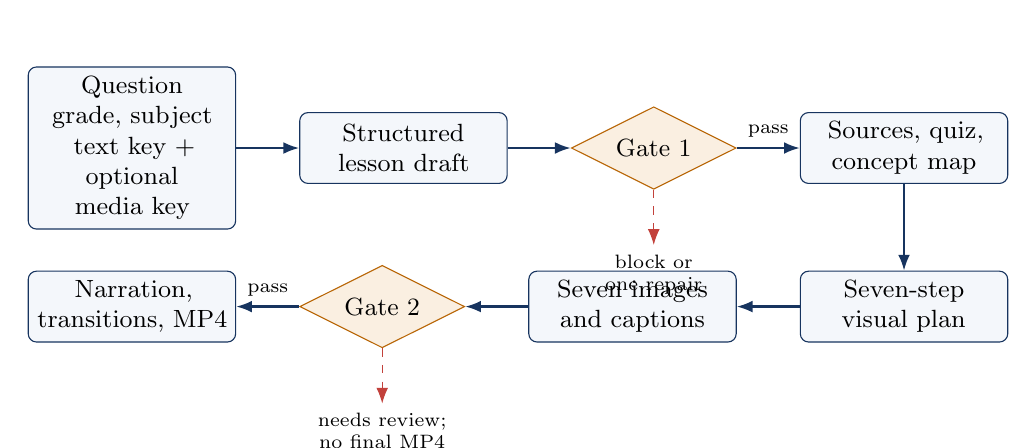
\begin{tikzpicture}[
 node distance=5mm and 8mm,
 box/.style={draw=navy,rounded corners=3pt,fill=pale,minimum height=9mm,text width=24mm,align=center,font=\small},
 gate/.style={diamond,draw=amber!85!black,fill=amber!12,aspect=2.0,align=center,font=\small},
 arrow/.style={-{Latex[length=2mm]},thick,draw=navy}
]
\node[box] (input) {Question\\grade, subject\\text key + optional media key};
\node[box,right=of input] (draft) {Structured\\lesson draft};
\node[gate,right=of draft] (g1) {Gate 1};
\node[box,right=of g1] (evidence) {Sources, quiz,\\concept map};
\node[box,below=11mm of evidence] (plan) {Seven-step\\visual plan};
\node[box,left=of plan] (images) {Seven images\\and captions};
\node[gate,left=of images] (g2) {Gate 2};
\node[box,left=of g2] (video) {Narration,\\transitions, MP4};
\draw[arrow] (input)--(draft);
\draw[arrow] (draft)--(g1);
\draw[arrow] (g1)--node[above,font=\scriptsize]{pass}(evidence);
\draw[arrow] (evidence)--(plan);
\draw[arrow] (plan)--(images);
\draw[arrow] (images)--(g2);
\draw[arrow] (g2)--node[above,font=\scriptsize]{pass}(video);
\draw[-{Latex[length=2mm]},draw=red,dashed] (g1.south) -- ++(0,-7mm) node[below,font=\scriptsize,align=center]{block or\\one repair};
\draw[-{Latex[length=2mm]},draw=red,dashed] (g2.south) -- ++(0,-7mm) node[below,font=\scriptsize,align=center]{needs review;\\no final MP4};
\end{tikzpicture}
\caption{Production architecture. The ordering is also a spending policy: text is checked before image calls, and frames are checked before final composition.}
\label{fig:architecture}
\end{figure}

The application stores explicit status rather than a single success flag. Gate 2 can be waiting, blocked by Gate 1, not applicable to a text-only lesson, incomplete because media failed, passed, or marked for review. This prevents a narration failure from erasing a completed visual audit.

\section{Why We Use a Staged Cascade}

Suppose a text check costs $C_T$, research costs $C_R$, images cost $C_I$, and narration plus composition costs $C_V$. Let $p_1$ be the fraction of drafts that pass Gate 1 and $p_2$ the fraction of frame sets that pass Gate 2. A simplified expected variable cost is
\begin{equation}
  \mathbb{E}[C]=C_T+p_1(C_R+C_I)+p_1p_2C_V.
  \label{eq:expected-cost}
\end{equation}
The equation uses multiplication for a simple reason: the video stage is reached only when both earlier events occur. If a draft fails, we do not buy images for it. If its images fail, we do not pretend the final video is approved.

\begin{figure}[H]
\centering
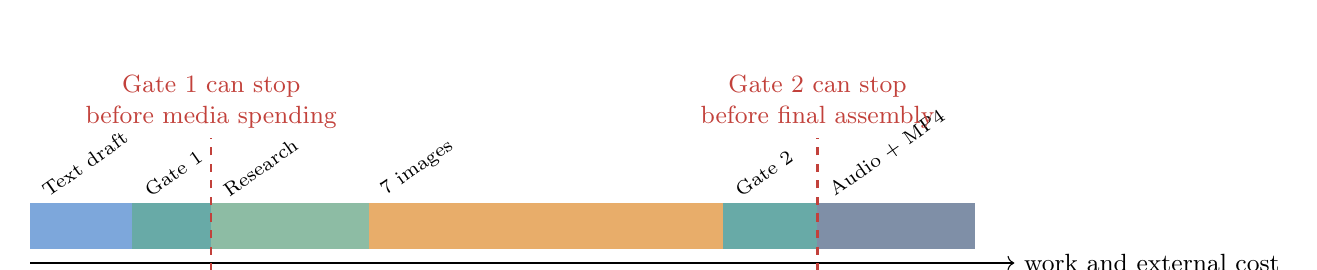
\begin{tikzpicture}[x=1cm,y=0.72cm,font=\small]
\draw[->] (0,0)--(12.5,0) node[right]{work and external cost};
\foreach \x/\w/\c/\lab in {0/1.3/blue!65/Text draft,1.3/1.0/teal!65/Gate 1,2.3/2.0/green!55/Research,4.3/4.5/amber!60/7 images,8.8/1.2/teal!65/Gate 2,10.0/2.0/navy!55/Audio + MP4}{
  \fill[\c] (\x,0.25) rectangle +(\w,0.8);
  \node[rotate=35,anchor=west,font=\scriptsize] at (\x+0.08,1.15) {\lab};
}
\draw[red,dashed,thick] (2.3,-0.15)--(2.3,2.2) node[above,align=center]{Gate 1 can stop\\before media spending};
\draw[red,dashed,thick] (10,-0.15)--(10,2.2) node[above,align=center]{Gate 2 can stop\\before final assembly};
\end{tikzpicture}
\caption{Qualitative cost path. Segment widths illustrate relative workflow weight; they are not provider prices. Actual prices and latency vary by model and date.}
\label{fig:cost}
\end{figure}

The cascade also improves diagnosis. A local readability warning, a factual rubric failure, a dark frame, and a sequence-continuity problem should not all appear as ``generation failed.'' Each belongs to a different stage and suggests a different correction.

\section{Mathematical Design Questions}

The project uses mathematics as a design language, not as decoration. Each formula answers a practical question that a high-school student can follow:

\begin{table}[H]
\centering
\small
\begin{tabularx}{\linewidth}{@{}p{0.32\linewidth}Y p{0.19\linewidth}@{}}
\toprule
\textbf{Question} & \textbf{Mathematical conclusion} & \textbf{Detailed proof} \\
\midrule
Can a weighted score leave the interval $[0,1]$? & No, when every component is in $[0,1]$, weights are nonnegative, and weights sum to one. & Proposition~\ref{prop:convex} \\
Can a high average hide a serious factual weakness? & Yes. A mandatory accuracy rule is therefore separate from the average. & Proposition~\ref{prop:noncomp} \\
Why must all seven frames pass? & A mean can hide one weak frame, and the chance of at least one defect rises with the number of frames. & Proposition~\ref{prop:allframe} \\
Which check should run first? & For two independent screening stages, compare cost per rejection probability, $c/r$. & Theorem~\ref{thm:ordering} \\
Why process frame diagnostics in parallel? & Parallel time is no greater than sequential time; with equal jobs and four workers, seven jobs need at least two waves. & Proposition~\ref{prop:parallel} \\
Does timing allocation create or lose duration? & No. The scene-duration formula sums exactly to the chosen total and preserves the per-scene floor. & Proposition~\ref{prop:timing} \\
\bottomrule
\end{tabularx}
\caption{The main mathematical questions behind the production design. The appendices use only algebra, averages, inequalities, elementary probability, and graphs.}
\label{tab:math-roadmap}
\end{table}

A proof in this paper establishes a property of the \emph{implemented formula under stated assumptions}. It does not prove that a model response is true, that a student learned, or that a chosen threshold is optimal. Those questions require observations and evaluation data.
\section{Gate 1: Explanation Review}

\subsection{Local screen}

The local screen checks four transparent conditions: the explanation contains 70--420 alphabetic words; it includes at least one important term from the question when such terms exist; and its mean sentence length is no more than 27 words. These values are engineering defaults for a focused lesson, not universal reading-level standards. The gate reports the violated condition instead of hiding it behind a classifier label.

\subsection{Semantic rubric and bounded repair}

A semantic reviewer scores accuracy, completeness, logical flow, grade fit, and clarity from 1 to 4. Accuracy must equal 4, and every other dimension must be at least 3. When the first review fails but returns a revision, the system allows one repair and one recheck. The maximum of two semantic calls bounds the loop.

\begin{figure}[H]
\centering
\resizebox{0.96\linewidth}{!}{%
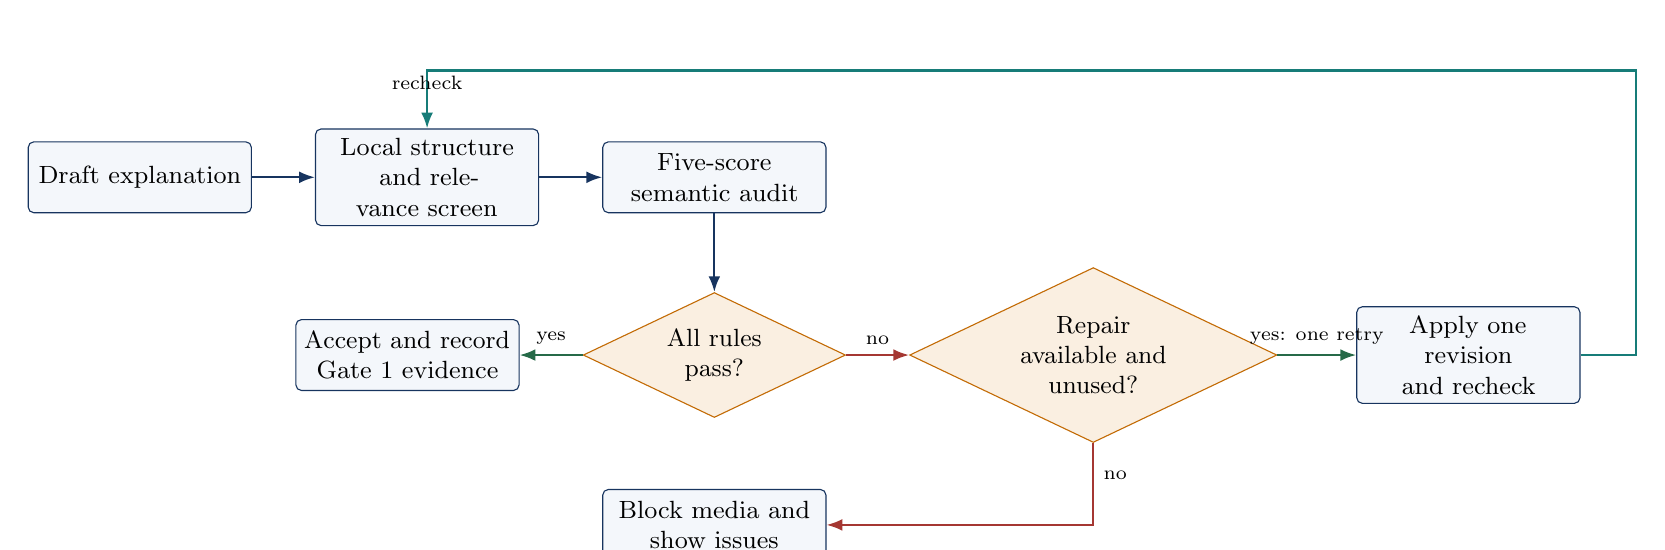
\begin{tikzpicture}[
 node distance=7mm and 8mm,
 proc/.style={draw=navy,rounded corners=2pt,fill=pale,text width=26mm,minimum height=9mm,align=center,font=\small},
 dec/.style={diamond,draw=amber!90!black,fill=amber!12,aspect=2.1,align=center,font=\small},
 arr/.style={-{Latex[length=2mm]},thick,draw=navy},
 yesarr/.style={arr,draw=green!80!black},
 noarr/.style={arr,draw=red!85!black},
 retryarr/.style={arr,draw=teal}
]
\node[proc] (draft) {Draft explanation};
\node[proc,right=of draft] (local) {Local structure\\and relevance screen};
\node[proc,right=of local] (rubric) {Five-score\\semantic audit};
\node[dec,below=10mm of rubric] (pass) {All rules\\pass?};
\node[proc,left=of pass] (accept) {Accept and record\\Gate 1 evidence};
\node[dec,right=of pass] (repair) {Repair\\available and\\unused?};
\node[proc,right=10mm of repair] (revise) {Apply one revision\\and recheck};
\node[proc,below=9mm of pass] (block) {Block media and\\show issues};
\draw[arr] (draft)--(local); \draw[arr] (local)--(rubric); \draw[arr] (rubric)--(pass);
\draw[yesarr] (pass)--node[above,font=\scriptsize]{yes}(accept);
\draw[noarr] (pass)--node[above,font=\scriptsize]{no}(repair);
\draw[yesarr] (repair)--node[above,font=\scriptsize]{yes: one retry}(revise);
\draw[noarr] (repair.south) |- node[pos=0.2,right,font=\scriptsize]{no} (block.east);
\draw[retryarr] (revise.east) -- ++(7mm,0) |- ($(rubric.north)+(0,9mm)$) -| node[pos=0.75,above,font=\scriptsize]{recheck} (local.north);
\end{tikzpicture}%
}
\caption{Gate 1 decision graph. The loop is bounded to prevent indefinite self-revision.}
\label{fig:gate1}
\end{figure}

If the five scores are $s_d\in\{1,2,3,4\}$, the displayed normalized score is
\begin{equation}
  S_1=\frac{1}{5}\sum_{d=1}^{5}\frac{s_d}{4}.
\end{equation}
A score of $S_1=0.90$ is not sufficient by itself. The logical pass rule still requires maximum accuracy and no failed local check. Appendix~\ref{app:math} gives the exact indicator form and examples.

\subsection{Why the saved text classifier is not the production judge}

The repository retains DistilBERT, BERT, and RoBERTa experiments. BERT introduced bidirectional transformer pretraining, RoBERTa revised its training recipe, and DistilBERT compressed a larger teacher model \citep{devlin2019bert,liu2019roberta,sanh2019distilbert}. Our saved models classify pedagogical error categories on the experiment dataset. That is useful offline evidence, but it is not the same task as verifying an arbitrary new explanation. We therefore report those models as baselines and use the narrower, inspectable cascade in production.
\section{Gate 2: Visual Review}

\subsection{Parallel technical checks}

Gate 2 receives seven ordered frames. For each frame, it measures width, height, mean grayscale brightness, grayscale contrast, edge variation, and variation in the lower caption band. Four worker threads process frames in parallel. Five normalized component scores then represent resolution, exposure, contrast, detail, and caption-band readability. Their weighted sum produces a technical frame score $t_i\in[0,1]$.

The local stage uses a strict all-frame rule. Its mean must be adequate, and every required frame must meet the technical threshold $0.42$. This is important because an average can hide one unusable teaching step. If any frame fails, the system stops before a vision-model call.

\subsection{One semantic contact-sheet review}

When the technical stage passes and a compatible vision client is available, the frames are resized into one ordered contact sheet. One call scores semantic accuracy, teaching alignment, sequence continuity, legibility, and visual load from 1 to 4. Semantic accuracy must equal 4 and all other dimensions must be at least 3. The combined display score is
\begin{equation}
  S_2=0.35T+0.65M,
  \label{eq:gate2}
\end{equation}
where $T$ is mean technical quality and $M$ is normalized semantic quality. The larger semantic weight expresses an engineering priority: a sharp, bright image is still a poor teaching image if it communicates the wrong idea. The weights and thresholds were not learned from classroom outcomes and should be recalibrated when a suitable labeled dataset becomes available.

\begin{figure}[H]
\centering
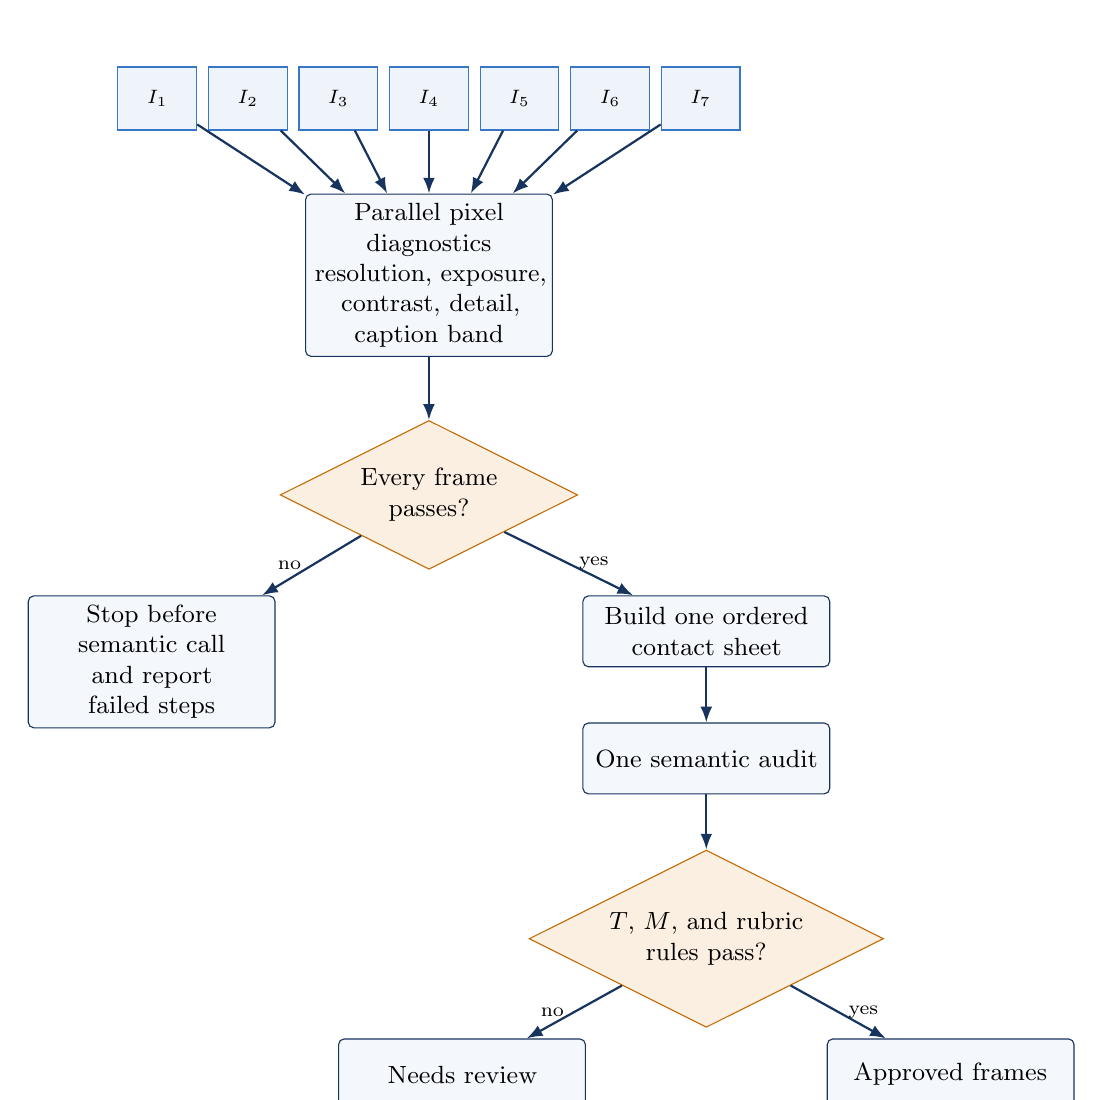
\begin{tikzpicture}[
 node distance=5mm and 7mm,
 frame/.style={draw=blue,fill=blue!8,minimum width=10mm,minimum height=8mm,font=\scriptsize},
 proc/.style={draw=navy,rounded corners=2pt,fill=pale,text width=29mm,minimum height=9mm,align=center,font=\small},
 dec/.style={diamond,draw=amber!90!black,fill=amber!12,aspect=2.0,align=center,font=\small},
 arr/.style={-{Latex[length=2mm]},thick,draw=navy}
]
\foreach \i in {1,...,7}{\node[frame] (f\i) at ({(\i-4)*1.15},0) {$I_{\i}$};}
\node[proc,below=8mm of f4] (parallel) {Parallel pixel diagnostics\\resolution, exposure, contrast, detail, caption band};
\node[dec,below=8mm of parallel] (tech) {Every frame\\passes?};
\node[proc,below left=8mm and 10mm of tech] (stop) {Stop before semantic call\\and report failed steps};
\node[proc,below right=8mm and 10mm of tech] (sheet) {Build one ordered\\contact sheet};
\node[proc,below=7mm of sheet] (vision) {One semantic audit};
\node[dec,below=7mm of vision] (final) {$T$, $M$, and rubric\\rules pass?};
\node[proc,below left=7mm and 4mm of final] (review) {Needs review};
\node[proc,below right=7mm and 4mm of final] (approved) {Approved frames};
\foreach \i in {1,...,7}{\draw[arr] (f\i)--(parallel);}
\draw[arr] (parallel)--(tech);
\draw[arr] (tech)--node[left,font=\scriptsize]{no}(stop);
\draw[arr] (tech)--node[right,font=\scriptsize]{yes}(sheet);
\draw[arr] (sheet)--(vision); \draw[arr] (vision)--(final);
\draw[arr] (final)--node[left,font=\scriptsize]{no}(review);
\draw[arr] (final)--node[right,font=\scriptsize]{yes}(approved);
\end{tikzpicture}
\caption{Gate 2 decision graph. Pixel diagnostics screen rendering failures; the contact sheet addresses meaning and continuity.}
\label{fig:gate2}
\end{figure}

\subsection{Why CLIP remains an offline comparison}

CLIP learns an image--text representation through contrastive pretraining and can measure whether an image and caption are close in its embedding space \citep{radford2021learning}. Our saved Gate 2 experiments compare cosine thresholding with linear and multilayer probes on aligned and mismatched Flickr8k pairs \citep{hodosh2013framing}. This benchmark asks whether a caption matches an image. Production Gate 2 also asks whether labels are readable, exposure is usable, the sequence remains coherent, and the visual teaches the approved explanation. Because the tasks differ, we do not present the CLIP benchmark as a production certification.

\section{From Approved Frames to Video}

\subsection{Why we removed direct text-to-video generation}

We removed the direct video path for three reasons. First, a generated clip is harder to inspect at the level of individual teaching steps. Second, it can change objects, labels, or causal relations over time. Third, its cost is difficult to control in a classroom workflow. The still-image route creates seven explicit checkpoints and allows visual-only regeneration without rewriting an approved explanation.

\subsection{Storyboard contract}

The planner produces a shared scene bible and seven ordered steps. Each step states its teaching goal, retained objects, additions, removals, labels, and misconceptions to avoid. The image prompt includes the same visual style, layout zones, typography, color assignments, and canonical explanation. A fixed lower band is reserved for captions. These constraints implement coherence and signaling as engineering rules rather than asking the image model to rediscover them for every frame \citep{mayer2021handbook}.

\begin{figure}[H]
\centering
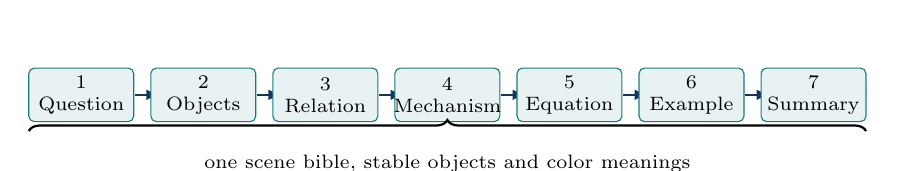
\begin{tikzpicture}[x=1.55cm,y=1cm,font=\small]
\foreach \i/\lab in {1/Question,2/Objects,3/Relation,4/Mechanism,5/Equation,6/Example,7/Summary}{
  \draw[rounded corners=2pt,fill=teal!10,draw=teal] (\i-1,0) rectangle +(0.86,0.68);
  \node[font=\scriptsize,align=center] at (\i-0.57,0.34) {\i\\\lab};
  \ifnum\i<7 \draw[-{Latex[length=1.8mm]},navy,thick] (\i-0.13,0.34)--(\i+0.08,0.34); \fi
}
\draw[decorate,decoration={brace,amplitude=4pt},thick] (0,-0.12)--(6.86,-0.12);
\node[below,font=\scriptsize] at (3.43,-0.3) {one scene bible, stable objects and color meanings};
\end{tikzpicture}
\caption{A seven-scene instructional timeline. Labels describe roles, not a mandatory subject template; the planner adapts them to the question.}
\label{fig:timeline}
\end{figure}

\subsection{Narration-aware timing and composition}

The system estimates or measures narration length, gives every scene at least 3.2 seconds, and allocates remaining time by caption word count. Frames are fitted to a 16:9 canvas over a blurred background so content is not cropped. A restrained 1.8\% Ken Burns movement alternates direction, and adjacent scenes cross-fade. The video is encoded as H.264 with CRF 18, browser-compatible \code{yuv420p}, and fast-start metadata. Narration is normalized toward $-16$ LUFS with a $-1.5$ dB true-peak ceiling when the FFmpeg filter is available. Appendix~\ref{app:math} gives the timing equation.

\section{Student-Facing Lesson Structure}

The generated bundle is rendered as six views:
\begin{enumerate}
  \item \textbf{Lesson:} objective, explanation, key ideas, worked example, common mistake, and quick check.
  \item \textbf{Concept map:} prerequisites, applications, contrasts, and next topics.
  \item \textbf{Evidence and sources:} a grounded synthesis, source-by-source notes, and evidence limits.
  \item \textbf{Practice:} five multiple-choice items with answer explanations and missed-concept guidance.
  \item \textbf{Learning library:} deterministic links to established platforms rather than model-invented URLs.
  \item \textbf{Quality report:} gate path, score, latency, issues, repairs, and model-call count.
\end{enumerate}

Markdown and common LaTeX wrappers are normalized before Streamlit renders them. This prevents a useful equation such as $F=ma$ from appearing as raw control characters. The normalizer preserves paragraphs and lists instead of flattening the lesson into one line.

\subsection{Useful waiting time rather than an empty spinner}

Model and image calls can take long enough for a learner to disengage. The deployed interface therefore reports a stage label and a monotone progress fraction. During the seven-frame loop it reports when each illustration starts and finishes. The display does \emph{not} claim to predict seconds remaining; provider queues and retries make such a prediction unreliable.

The same panel shows one short study action selected from a small code-controlled library. Drafting tips ask the learner to predict or recall; gate tips ask about units, assumptions, and counterexamples; research tips ask the learner to compare sources; frame tips ask the learner to follow arrows or explain visual change; composition tips recommend retrieval rather than passive replay. The selector uses only stage, grade, subject text, and frame number. It does not infer emotion, attention, disability, or ability. Appendix~\ref{app:progress} proves that the displayed media progress never moves backward and explains the modulo selector used for tips.

\subsection{Connected concepts as an interactive directed graph}

The text model proposes five short topic connections. The program normalizes each relationship into one of five roles: prerequisite, application, contrast, next step, or related concept. It then discards any model-generated URL and attaches sources using deterministic subject mappings to platforms such as OpenStax, Khan Academy, GeoGebra, PhET, and MDN. This separation is important: the model proposes \emph{what may be related}; code-controlled mappings decide \emph{where a learner may click}.

The current view is not a static star diagram. A horizontal control filters learning roles. A focus selector and a \emph{Next link} button move through topics. The focused topic shows why it matters, trusted links, and a relationship-specific challenge. A learner may mark ``I can explain this link,'' and a progress bar displays the number marked out of the total. This is a self-report and navigation aid, not a mastery diagnosis.

\begin{figure}[H]
\centering
\resizebox{0.98\linewidth}{!}{%
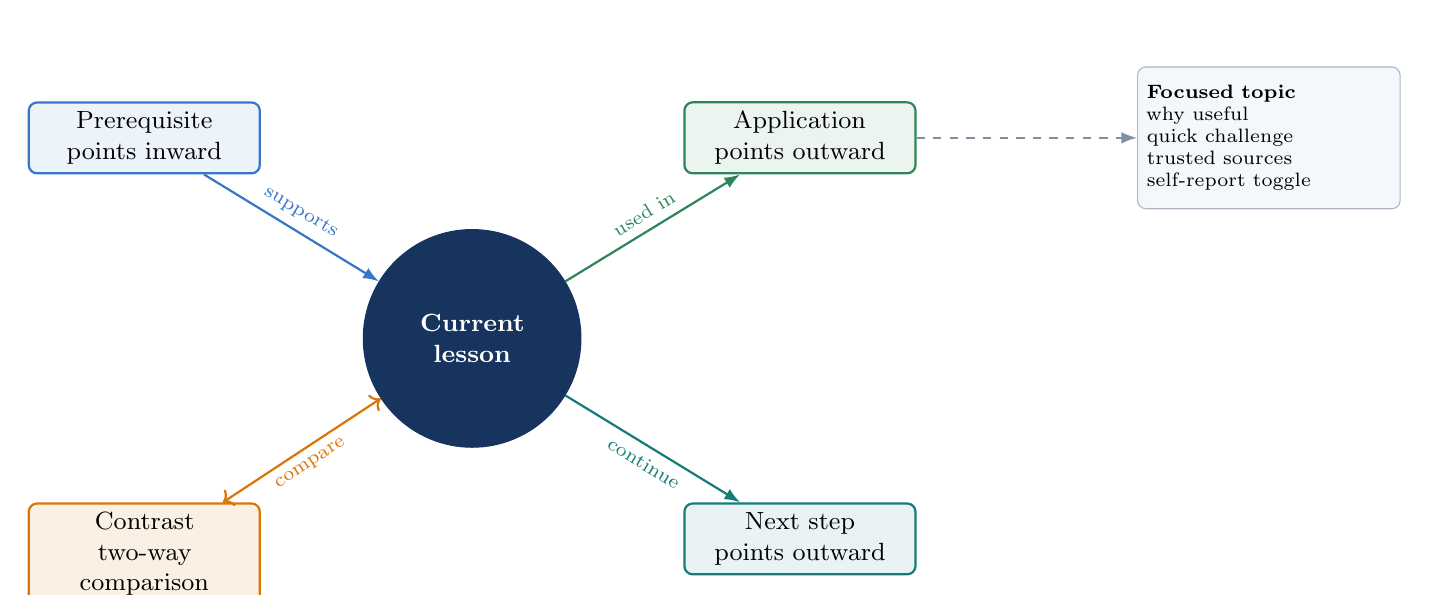
\begin{tikzpicture}[
 node distance=11mm and 17mm,
 core/.style={circle,draw=navy,fill=navy,text=white,text width=24mm,align=center,minimum size=22mm,font=\small\bfseries},
 topic/.style={rectangle,rounded corners=3pt,text width=27mm,align=center,minimum height=9mm,font=\small,thick},
 panel/.style={rectangle,rounded corners=3pt,draw=navy!35,fill=pale,text width=31mm,align=left,minimum height=18mm,font=\scriptsize},
 edge/.style={-{Latex[length=2mm]},thick}
]
\node[core] (c) {Current\\lesson};
\node[topic,draw=blue,fill=blue!9,above left=of c] (p) {Prerequisite\\points inward};
\node[topic,draw=green,fill=green!9,above right=of c] (a) {Application\\points outward};
\node[topic,draw=amber,fill=amber!11,below left=of c] (d) {Contrast\\two-way comparison};
\node[topic,draw=teal,fill=teal!9,below right=of c] (n) {Next step\\points outward};
\node[panel,right=28mm of a] (focus) {\textbf{Focused topic}\\why useful\\quick challenge\\trusted sources\\self-report toggle};
\draw[edge,blue] (p)--node[above,sloped,font=\scriptsize]{supports}(c);
\draw[edge,green] (c)--node[above,sloped,font=\scriptsize]{used in}(a);
\draw[edge,amber,<->] (c)--node[below,sloped,font=\scriptsize]{compare}(d);
\draw[edge,teal] (c)--node[below,sloped,font=\scriptsize]{continue}(n);
\draw[edge,navy!55,dashed] (a)--(focus);
\end{tikzpicture}
}
\caption{The deployed concept neighborhood encodes learning direction and connects the selected node to an interactive study panel. Filtering changes the displayed subgraph; it does not regenerate the lesson or make another model call.}
\label{fig:concept}
\end{figure}

Let the concept graph be $G=(V,E)$, where the current lesson and related topics are vertices and labeled relationships are directed edges. If a learner marks $m$ of $n$ related topics, the displayed self-report progress is $m/n$. Appendix~\ref{app:graph} proves its bounds and shows why adding one completed connection changes the bar by exactly $1/n$.
\section{Offline Checker Experiments}

The repository contains saved benchmark summaries for the earlier research checkers. Table~\ref{tab:benchmarks} reports the values used by the application's friendly experiment snapshot. Gate 1 and Gate 2 use different datasets and tasks, so their rows must not be ranked against one another.

\begin{table}[H]
\centering
\small
\begin{tabular}{@{}llrrrrr@{}}
\toprule
Gate & Method & Accuracy & Precision & Recall & F1 & AUROC \\
\midrule
1 & DistilBERT classifier & 0.9280 & 0.9444 & 0.9280 & 0.9284 & -- \\
1 & BERT classifier & 0.9253 & 0.9314 & 0.9253 & 0.9249 & -- \\
1 & RoBERTa classifier & 0.9653 & 0.9667 & 0.9653 & 0.9655 & -- \\
2 & CLIP cosine threshold & 0.9628 & 0.9474 & 0.9800 & 0.9634 & 0.9922 \\
2 & CLIP linear probe & 0.8756 & 0.8301 & 0.9444 & 0.8836 & 0.9555 \\
2 & CLIP MLP probe & 0.9517 & 0.9462 & 0.9578 & 0.9520 & 0.9885 \\
\bottomrule
\end{tabular}
\caption{Saved offline metrics. Gate 1 classifies pedagogical error types. Gate 2 classifies aligned versus mismatched Flickr8k pairs. ``--'' means AUROC was not retained in the summarized multiclass result.}
\label{tab:benchmarks}
\end{table}

\begin{figure}[H]
\centering
\begin{subfigure}{0.48\linewidth}
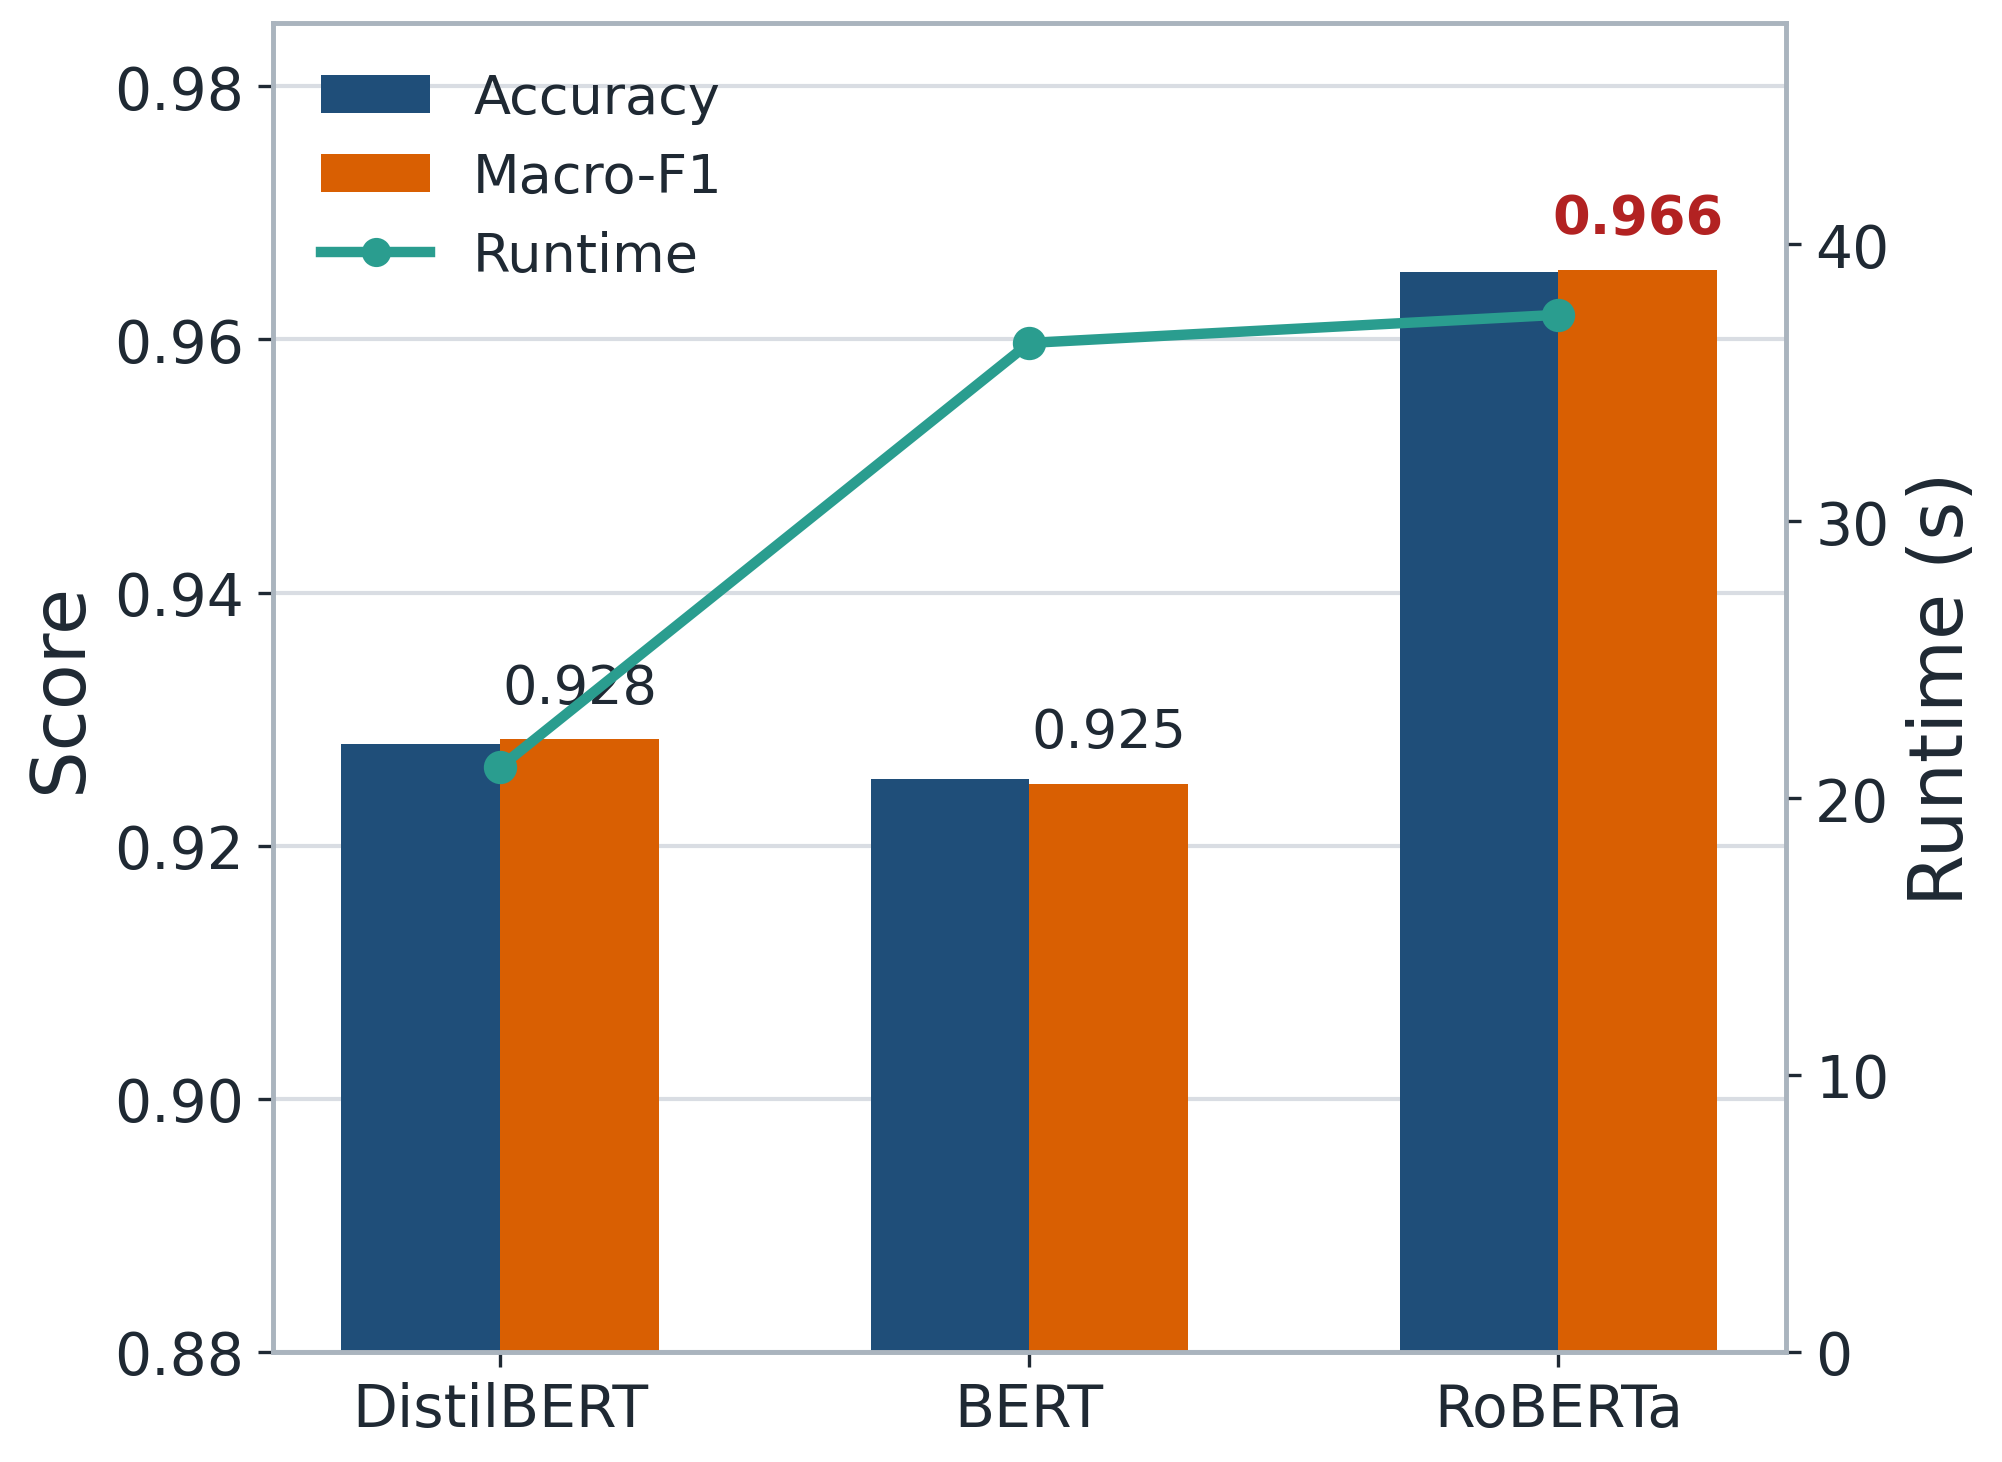
\includegraphics[width=\linewidth]{checker1_comparison_publication.png}
\caption{Gate 1 classifier comparison.}
\end{subfigure}\hfill
\begin{subfigure}{0.48\linewidth}
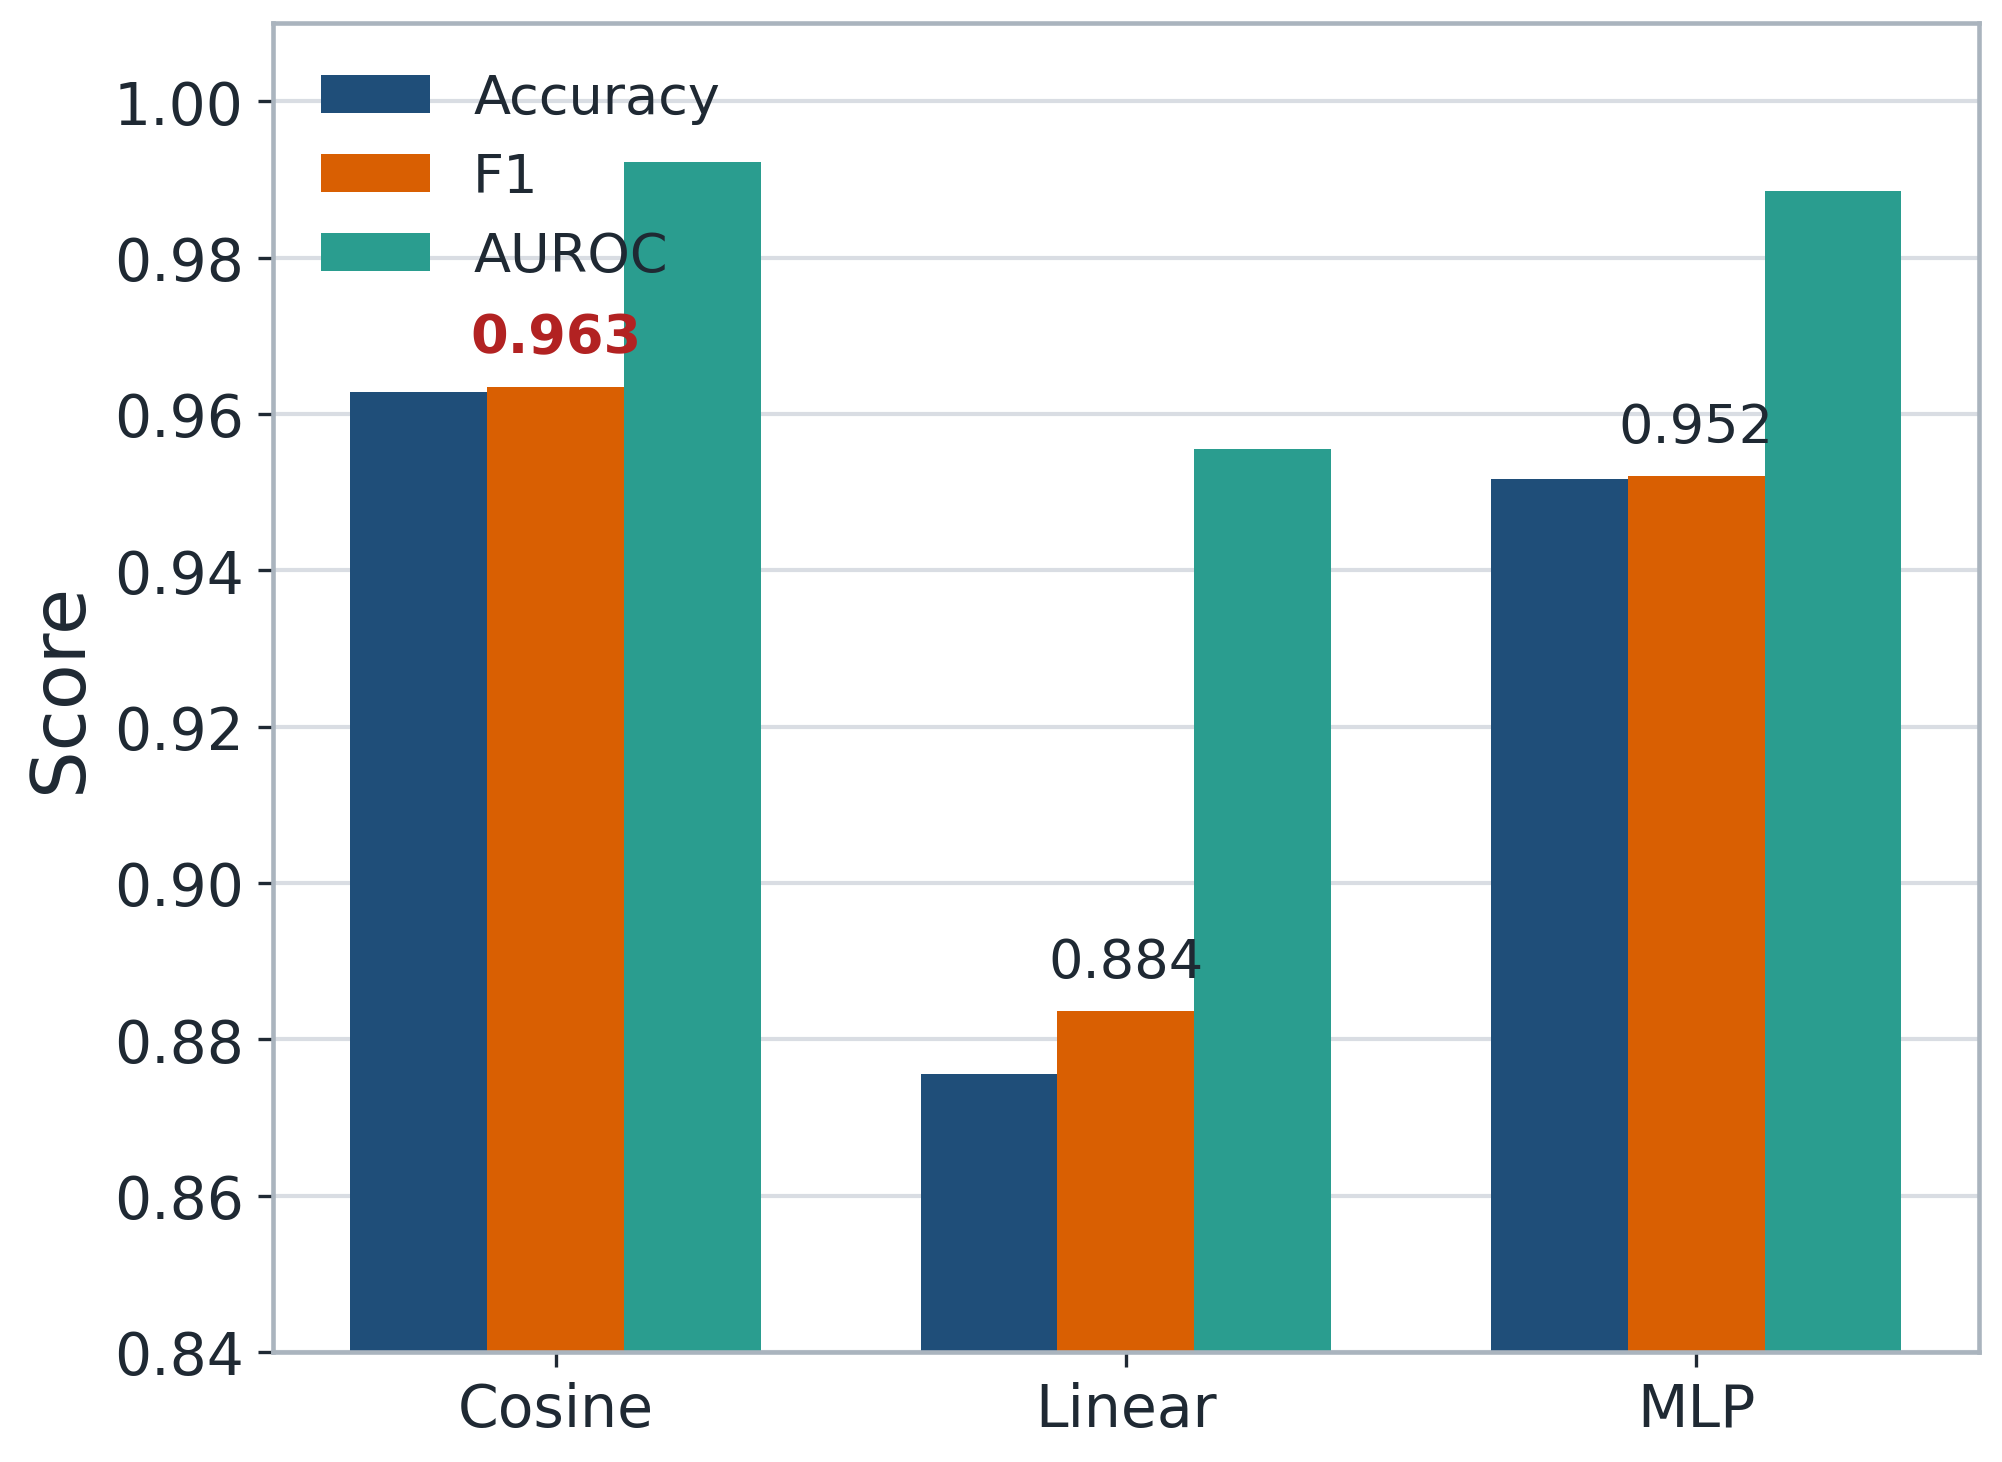
\includegraphics[width=\linewidth]{checker2_comparison_publication.png}
\caption{Gate 2 alignment comparison.}
\end{subfigure}
\caption{Offline experiment figures generated from repository records. These plots do not show live request latency or learning outcomes.}
\label{fig:offlineplots}
\end{figure}

The RoBERTa classifier has the highest saved Gate 1 F1. The untrained CLIP cosine threshold has the highest saved Gate 2 F1 and AUROC. This result illustrates why ``trained'' is not itself a deployment metric. We also consider task match, startup weight, latency, interpretability, and whether a baseline measures the product failure we need to catch.

\subsection{Metric interpretation}

Accuracy asks what fraction of all predictions were correct. Precision asks, among examples predicted positive, how many were positive. Recall asks, among all positive examples, how many were found. F1 is the harmonic mean of precision and recall. AUROC summarizes ranking across thresholds. Appendix~\ref{app:math} defines each quantity and gives a small confusion-matrix example. For imbalanced classes, accuracy alone can be misleading; this is why we retain multiple metrics \citep{fawcett2006roc}.

\section{Reproducible Local Setup}

\subsection{Requirements}

The production target is Python 3.12. The minimal application dependencies are OpenAI's Python SDK, Pillow, ImageIO, ImageIO-FFmpeg, Streamlit, Requests, and Graphviz. A local Graphviz executable may also be required for graph rendering. Research and training dependencies are isolated from the website requirements.

\subsection{Installation}

\begin{lstlisting}[language=bash]
git clone https://github.com/allanzhang721/AiLessonStudio.git
cd AiLessonStudio
python -m venv .venv
# Windows PowerShell
.venv\Scripts\Activate.ps1
# macOS or Linux: source .venv/bin/activate
python -m pip install --upgrade pip
python -m pip install -r requirements.txt
python -m pytest -q
python -m streamlit run streamlit_app.py
\end{lstlisting}

The app opens before a key is entered, but generation remains locked until the required fields are present. The first password field is always the text key. With OpenAI selected for text, that same key can be reused for research, images, visual review, and narration. With DeepSeek selected, the interface states that DeepSeek is text-only in this application. The learner may stop there and generate a written lesson, or open \emph{Add image API (optional)}. Only then does a second OpenAI image-key field appear; that optional key supplies images, the semantic visual audit, narration, and MP4 composition while DeepSeek continues to write the lesson.

\subsection{Directory map}

\begin{lstlisting}
streamlit_app.py              # production entrypoint
app_v2.py                     # complete Streamlit interface
pipeline/
  lesson_service.py           # bundle generation, research, sources
  quality_gates.py            # Gate 1
  frame_checker.py            # Gate 2
  planner.py                  # seven-scene plan
  image_pipeline.py           # frame generation
  video_pipeline.py           # timing, motion, audio, MP4
  markdown_render.py          # Markdown and LaTeX normalization
  gate_benchmarks.py          # small offline metric snapshot
tests/                        # deployment and regression tests
requirements.txt              # production dependencies
requirements-research.txt     # optional experiment dependencies
\end{lstlisting}

\subsection{Test protocol}

The production subset contains 33 executable tests at this paper version. It covers frame scoring and short-circuit behavior, explanation repair, provider routing, the conditional second-key Streamlit flow, concept relationship direction, progress callbacks, waiting-tip selection, source annotation conversion, schema normalization, Markdown and LaTeX handling, fail-fast plan validation, student-analysis helpers, narration arguments, audio-aware timing, and real H.264 encoding. Six additional research-only tests depend on experiment modules and data that are intentionally not shipped with the lightweight deployment checkout. The production command is:

\begin{lstlisting}[language=bash]
python -m pytest -q tests \
  --ignore=tests/test_checker1_research.py \
  --ignore=tests/test_checker2_research.py
\end{lstlisting}

A passing unit suite establishes that the code meets the tested contracts. It does not establish educational effectiveness. A publication evaluation should additionally include expert factual review, student comprehension measures, accessibility review, cost records, and failure analysis.
\section{Deployment, Privacy, and Operational Boundaries}

\begin{figure}[H]
\centering
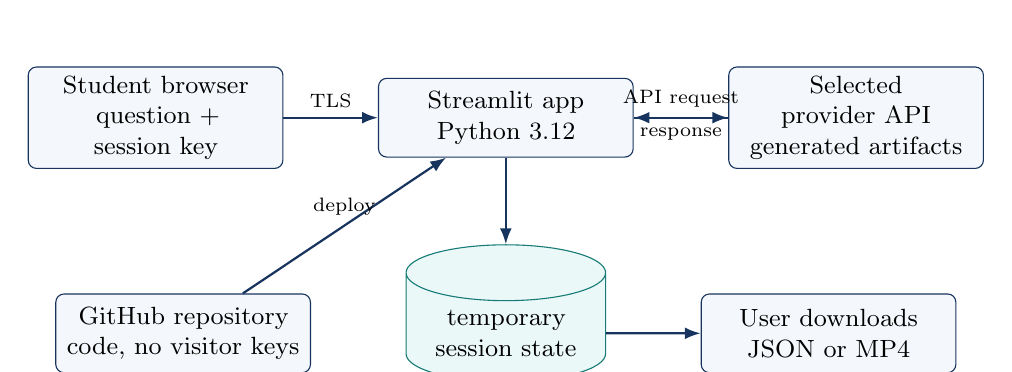
\begin{tikzpicture}[
 node distance=7mm and 12mm,
 box/.style={draw=navy,rounded corners=3pt,fill=pale,text width=30mm,minimum height=10mm,align=center,font=\small},
 store/.style={cylinder,shape border rotate=90,aspect=0.28,draw=teal,fill=soft,text width=23mm,minimum height=13mm,align=center,font=\small},
 arr/.style={-{Latex[length=2mm]},thick,draw=navy}
]
\node[box] (browser) {Student browser\\question + session key};
\node[box,right=of browser] (streamlit) {Streamlit app\\Python 3.12};
\node[box,right=of streamlit] (provider) {Selected provider API\\generated artifacts};
\node[store,below=11mm of streamlit] (state) {temporary\\session state};
\node[box,left=of state] (github) {GitHub repository\\code, no visitor keys};
\node[box,right=of state] (download) {User downloads\\JSON or MP4};
\draw[arr] (browser)--node[above,font=\scriptsize]{TLS}(streamlit);
\draw[arr] (streamlit)--node[above,font=\scriptsize]{API request}(provider);
\draw[arr] (provider)--node[below,font=\scriptsize]{response}(streamlit);
\draw[arr] (streamlit)--(state);
\draw[arr] (github)--node[above,font=\scriptsize]{deploy}(streamlit);
\draw[arr] (state)--(download);
\end{tikzpicture}
\caption{Deployment and data path. The project does not intentionally persist visitor keys; external providers still receive the requests authorized by those keys.}
\label{fig:deployment}
\end{figure}

The public deployment uses the \href{https://github.com/allanzhang721/AiLessonStudio}{AiLessonStudio repository}. Its production coordinates are branch \texttt{agent/}\allowbreak\texttt{streamlit-production}, entrypoint \texttt{streamlit\_app.py}, and Python 3.12. Streamlit Community Cloud installs dependencies from the repository and supports configuration of Python and secrets through its deployment settings \citep{streamlitDeploy,streamlitSecrets}. The current visitor flow does not require a repository secret because the visitor provides a session text key and, only when pairing a text-only provider with media, an optional session image key.

The password-style field reduces accidental display but is not a complete security boundary. The key is passed to the chosen provider client. Students should use restricted keys, set provider-side budgets, avoid entering personal information in prompts, and revoke a key they believe was exposed. School deployments should perform their own privacy, consent, procurement, and retention review.

\section{Source and Figure Provenance}

Table~\ref{tab:provenance} records where each kind of paper evidence comes from. This is important because a system diagram, an experiment plot, and an external research claim have different evidentiary status.

\begin{table}[H]
\centering
\small
\begin{tabularx}{\linewidth}{@{}p{0.25\linewidth}Y Y@{}}
\toprule
\textbf{Artifact} & \textbf{Source} & \textbf{Interpretation} \\
\midrule
Figures~\ref{fig:architecture}--\ref{fig:deployment} & Drawn in TikZ from the production source code and deployment configuration & Explanatory system diagrams; not experimental observations \\
Figure~\ref{fig:offlineplots} & Repository plotting outputs and saved benchmark values & Offline method comparison on recorded tasks \\
Table~\ref{tab:benchmarks} & \code{pipeline/gate\_benchmarks.py} & Distilled values used by the public dashboard \\
Gate, timing, progress, and graph equations & \code{quality\_gates.py}, \code{frame\_checker.py}, \code{pipeline.py}, \code{video\_pipeline.py}, and \code{lesson\_service.py} & Exact implementation or direct algebraic consequence as of the paper version \\
Learning rationale & Cited books, peer-reviewed articles, and public standards & Motivation for design choices, not a direct evaluation of this app \\
Setup instructions & Repository files and official Streamlit documentation & Reproducibility and deployment procedure \\
\bottomrule
\end{tabularx}
\caption{Evidence and figure provenance. No generated stock artwork is used in the technical diagrams.}
\label{tab:provenance}
\end{table}

\section{Limitations and Threats to Validity}

\paragraph{Shared-model bias.} A generator and semantic reviewer from related model families can share mistakes. The second call is a structured audit, not independent expert replication.

\paragraph{Proxy measurements.} Brightness, contrast, and edge variation detect technical defects but do not establish scientific correctness. Likewise, an image--caption benchmark does not measure the learning value of a seven-frame lesson.

\paragraph{Threshold selection.} The production thresholds are transparent engineering defaults. They have not been calibrated on a representative sample of teacher-rated generated lessons. Appendix~\ref{app:thresholds} lists each threshold so it can be challenged and replaced.

\paragraph{Dataset mismatch.} Gate 1 offline models classify error categories. Gate 2 offline models use Flickr8k alignment. Neither dataset estimates the probability that a new lesson improves high-school comprehension.

\paragraph{Provider dependence.} Model behavior, availability, price, and policy can change. The paper records product logic rather than promising a permanent provider capability.

\paragraph{Accessibility and language.} The interface supports multiple output languages, but the structural word rules are based on English alphabetic tokens. Caption readability metrics do not replace screen-reader, color-contrast, hearing-access, or multilingual review.

\paragraph{No classroom trial.} We have not yet reported a randomized or controlled student study. The correct next publication step is an evaluation with teachers and learners, not stronger language about the current benchmarks.

\section{Recommended Publication Evaluation}

We recommend a preregistered evaluation with three layers.
\begin{enumerate}
  \item \textbf{Artifact review:} subject teachers rate factual accuracy, missing conditions, grade appropriateness, and diagram correctness for a stratified set of questions.
  \item \textbf{System review:} measure latency, provider cost, gate pass rate, repair rate, false blocks, missed errors, and failure recovery.
  \item \textbf{Learner study:} compare an approved text lesson, an approved text-plus-video lesson, and a textbook/control condition using immediate and delayed questions. Record prior knowledge and avoid claiming personalization from one quiz.
\end{enumerate}

For gate calibration, teachers should label individual failure types and final usability independently. We can then choose thresholds on a validation split and report confidence intervals on a held-out test split. Precision and recall should be reported for the harmful-artifact class because missing a bad lesson and unnecessarily blocking a good lesson have different costs.

\section{Conclusion}

We built \product\ as a staged lesson studio because generated educational artifacts fail in different ways and because later media stages are costly. Gate 1 checks the explanation before research and images. Gate 2 checks every frame before final composition. The video path keeps seven inspectable images, stable captions, controlled timing, per-frame progress, and a recoverable intermediate state. The current app also supports a DeepSeek text lesson with an optional OpenAI media connection, a directional concept neighborhood with study challenges and self-report progress, cited notes, misconceptions, practice, regeneration, and a visible quality report.

The central lesson is not that more checking guarantees truth. It is that narrow checks, placed at the right boundaries, make failures cheaper to detect and easier to explain. The offline classifiers remain useful comparisons. The live gates remain engineering controls. Teacher and student evaluation remains necessary. Keeping these statements separate makes the project easier to reproduce, criticize, and improve.

\appendix
\section{Mathematical Appendix: Why the Gates Have This Form}
\label{app:math}

This appendix is written for a student who knows percentages, averages, algebra, graphs, and elementary probability. We use proofs to establish properties of the code. We do not use a formula as evidence that the generated lesson is factually correct.

\subsection{Definitions and assumptions}

A score is \emph{normalized} when it lies between 0 and 1. A normalized score of 0.8 means 80\% of the available score; it does not automatically mean an 80\% probability of correctness. An indicator
\[
\ind{A}=\begin{cases}1,&A\text{ is true},\\0,&A\text{ is false}\end{cases}
\]
turns a logical rule into arithmetic. Products of indicators represent ``and'': the product is 1 only when every factor is 1.

Throughout the appendix, weights are nonnegative. Probabilistic examples state when independence is assumed. Costs are illustrative units unless a provider price sheet and date are supplied.

\subsection{Why normalized weighted averages stay normalized}

\begin{proposition}[Convex-score bound]
\label{prop:convex}
Let $x_1,\ldots,x_d\in[0,1]$ and let $w_1,\ldots,w_d\ge0$ with $\sum_{j=1}^d w_j=1$. Then
\[
S=\sum_{j=1}^d w_jx_j
\]
also satisfies $0\le S\le1$.
\end{proposition}

\begin{proof}
Because each $w_j$ and $x_j$ is nonnegative, every product $w_jx_j$ is nonnegative, so $S\ge0$. Also $x_j\le1$, hence $w_jx_j\le w_j$. Adding these inequalities gives
\[
S=\sum_jw_jx_j\le\sum_jw_j=1.
\]
Therefore $S\in[0,1]$.
\end{proof}

This simple result explains why Gate 2 weights sum to one. It also makes the displayed percentage interpretable without extra clipping after aggregation.

\begin{proposition}[Sensitivity of a weighted score]
If one component $x_k$ increases by $\Delta$ while all other components stay fixed, then $S$ increases by exactly $w_k\Delta$.
\end{proposition}

\begin{proof}
The new score is
\[
S'=\sum_{j\ne k}w_jx_j+w_k(x_k+\Delta)=S+w_k\Delta.
\]
Subtracting $S$ gives $S'-S=w_k\Delta$.
\end{proof}

Thus a weight is also a sensitivity coefficient. In Gate 2, a 0.10 improvement in semantic score changes the combined score by $0.65(0.10)=0.065$, whereas the same technical improvement changes it by $0.35(0.10)=0.035$.

\subsection{Gate 1: an average plus mandatory conditions}

Let
\[
\mathbf{s}=(s_a,s_c,s_l,s_g,s_r),\qquad s_j\in\{1,2,3,4\},
\]
represent accuracy, completeness, logical flow, grade fit, and readability. The displayed score is
\begin{equation}
S_1=\frac{s_a+s_c+s_l+s_g+s_r}{20}.
\label{eq:gate1-score}
\end{equation}
Let $J$ be the number of local structural issues and $b\in\{0,1\}$ the reviewer's explicit decision. The production pass rule is
\begin{equation}
P_1=\ind{J=0}\ind{s_a=4}\ind{\min(s_c,s_l,s_g,s_r)\ge3}\ind{b=1}.
\label{eq:gate1-pass}
\end{equation}

\begin{proposition}[A high mean cannot protect a mandatory dimension]
\label{prop:noncomp}
For the five Gate 1 dimensions, a lesson can score at least 0.95 while failing the required accuracy condition.
\end{proposition}

\begin{proof}
Choose $(s_a,s_c,s_l,s_g,s_r)=(3,4,4,4,4)$. Then
\[
S_1=\frac{3+4+4+4+4}{20}=\frac{19}{20}=0.95.
\]
However, $\ind{s_a=4}=0$, so the product in Equation~\eqref{eq:gate1-pass} is zero. The lesson fails even though its mean is high.
\end{proof}

The example is a counterexample to the rule ``accept whenever the average is high.'' It motivates a \emph{noncompensatory} rule: strength in style or completeness cannot cancel a factual weakness.

\begin{workedexample}
Scores $(4,3,3,4,3)$ give $S_1=17/20=0.85$. If $J=0$ and $b=1$, every indicator equals 1 and the explanation passes. If one local issue remains, the first factor becomes zero and the same semantic scores fail.
\end{workedexample}

The review makes one initial semantic call. It permits at most one revised call, so
\begin{equation}
N_{1}=1+\ind{\text{first review fails and returns a revision}}\le2.
\end{equation}
This is a direct proof of the call bound: an indicator can only be 0 or 1.

\subsection{Gate 2 technical normalization}

Define
\begin{equation}
\clip(x)=\max(0,\min(1,x)),\qquad
\rho(x;a,b)=\clip\left(\frac{x-a}{b-a}\right),\quad b>a.
\end{equation}
If $x\le a$, then $\rho=0$; if $a<x<b$, it rises linearly; if $x\ge b$, it equals 1. The clipping function therefore converts measurements with different units into comparable normalized components without allowing a very large measurement to exceed 1.

For frame $i$, let $w_i,h_i$ be dimensions, $\mu_i$ mean grayscale brightness, $\sigma_i$ grayscale contrast, $e_i$ edge variation, and $c_i$ lower-caption-band variation. The code computes
\begin{align}
r_i &= \begin{cases}1,&w_i\ge1200\text{ and }h_i\ge800,\\0.4,&\text{otherwise},\end{cases}\\
x_i &= \min\{\rho(\mu_i;18,70),\rho(255-\mu_i;18,70)\},\\
q_i &= \rho(\sigma_i;18,60),\\
d_i &= \rho(e_i;14,46),\\
b_i &= \rho(c_i;8,28),\\
t_i &=0.20r_i+0.20x_i+0.25q_i+0.25d_i+0.10b_i.
\label{eq:technical-frame}
\end{align}
Each component lies in $[0,1]$, and the weights sum to 1. Proposition~\ref{prop:convex} therefore proves $t_i\in[0,1]$.

\begin{workedexample}
For components $(1.00,0.80,0.70,0.60,0.90)$,
\[
t_i=0.20+0.16+0.175+0.15+0.09=0.775.
\]
The arithmetic is visible and reproducible. It does not prove that the diagram teaches the right idea; that is why a separate semantic audit follows.
\end{workedexample}

\subsection{Why every frame must pass}

For $n=7$ frames, define
\[
T=\frac1n\sum_{i=1}^nt_i,
\qquad
P_T=\ind{T\ge0.42}\prod_{i=1}^{n}\ind{t_i\ge0.42}.
\]

\begin{proposition}[All-frame equivalence]
\label{prop:allframe}
The product $\prod_i\ind{t_i\ge0.42}$ equals 1 if and only if every frame meets the technical threshold.
\end{proposition}

\begin{proof}
If every frame meets the threshold, every indicator is 1 and their product is 1. Conversely, if even one frame fails, its indicator is 0. A product containing a zero is zero. These are the only two cases.
\end{proof}

A mean alone can hide a weak teaching step. If six frames score 0.85 and one scores 0.30, then
\[
T=\frac{6(0.85)+0.30}{7}=\frac{5.40}{7}\approx0.771.
\]
The mean looks strong, but the seventh frame may break the explanation. The product rule catches it.

There is also a probability reason. Suppose, only for illustration, that each frame independently has defect probability $p$. The probability that no frame is defective is $(1-p)^7$. Therefore
\begin{equation}
\Pr(\text{at least one defective frame})=1-(1-p)^7.
\label{eq:any-defect}
\end{equation}
The proof uses the complement rule: ``at least one'' is the opposite of ``none.''

\begin{table}[H]
\centering
\begin{tabular}{@{}rrrrr@{}}
\toprule
Per-frame defect probability $p$ & 0.01 & 0.05 & 0.10 & 0.20 \\
\midrule
At least one defect in seven & 0.068 & 0.302 & 0.522 & 0.790 \\
\bottomrule
\end{tabular}
\caption{Illustrative values of $1-(1-p)^7$. Independence is an assumption for this calculation, not a measured property of generated frames.}
\end{table}

\begin{figure}[H]
\centering
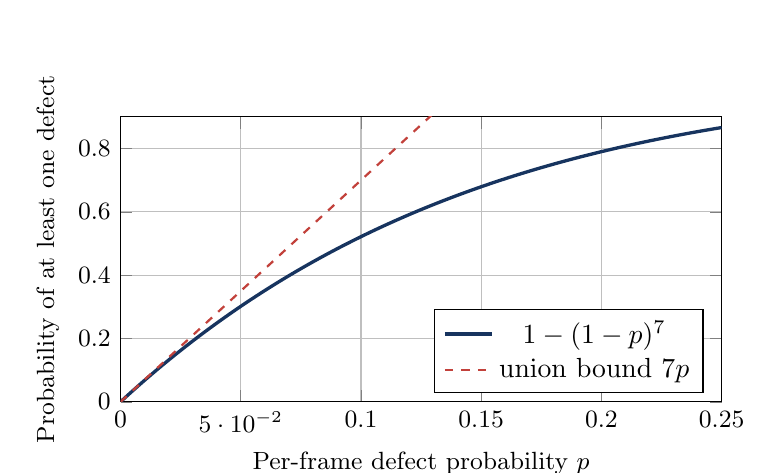
\begin{tikzpicture}
\begin{axis}[
 width=0.76\linewidth,height=5.2cm,
 xlabel={Per-frame defect probability $p$},
 ylabel={Probability of at least one defect},
 xmin=0,xmax=0.25,ymin=0,ymax=0.9,
 grid=major,legend pos=south east,
 tick label style={font=\small},label style={font=\small}
]
\addplot[navy,very thick,domain=0:0.25,samples=100]{1-(1-x)^7};
\addlegendentry{$1-(1-p)^7$}
\addplot[red,dashed,thick,domain=0:0.142857,samples=60]{7*x};
\addlegendentry{union bound $7p$}
\end{axis}
\end{tikzpicture}
\caption{Seven opportunities for failure make a per-frame check important. Without independence, the union bound still gives $\Pr(\text{any defect})\le7p$ when every frame has defect probability at most $p$.}
\label{fig:defect-probability}
\end{figure}

\subsection{Gate 2 semantic score and final rule}

Let $v_k\in\{1,2,3,4\}$ score semantic accuracy, teaching alignment, continuity, legibility, and visual load. Then
\begin{equation}
M=\frac1{20}\sum_{k=1}^5v_k,
\qquad
S_2=0.35T+0.65M.
\end{equation}
Because $T,M\in[0,1]$, Proposition~\ref{prop:convex} proves $S_2\in[0,1]$. If $v_a$ is semantic accuracy and $b_2$ the reviewer's Boolean result, the exact decision is
\begin{equation}
P_2=P_T\ind{v_a=4}\ind{\min_kv_k\ge3}\ind{b_2=1}\ind{S_2\ge0.65}.
\end{equation}

For $T=0.78$ and scores $(4,3,3,4,3)$, $M=17/20=0.85$ and
\[
S_2=0.35(0.78)+0.65(0.85)=0.8255.
\]
The set passes only if the other indicator rules also equal 1. Again, a combined score summarizes quality but does not replace a mandatory accuracy condition.

\subsection{Why a cheap effective gate should come early}

The production pipeline has dependency constraints: Gate 2 cannot run before images exist. Within the set of checks that could inspect the same item, elementary algebra gives an ordering rule.

\begin{theorem}[Two-check ordering rule]
\label{thm:ordering}
Suppose check $A$ costs $c_A>0$ and rejects a fraction $r_A>0$, while check $B$ costs $c_B>0$ and rejects a fraction $r_B>0$. A rejected item stops. Running $A$ before $B$ has no larger expected checking cost than running $B$ before $A$ exactly when
\begin{equation}
\frac{c_A}{r_A}\le\frac{c_B}{r_B}.
\label{eq:cost-rejection}
\end{equation}
\end{theorem}

\begin{proof}
With $A$ first, we always pay $c_A$ and pay $c_B$ only for the fraction $1-r_A$ that continues:
\[
E_{A\to B}=c_A+(1-r_A)c_B.
\]
Similarly,
\[
E_{B\to A}=c_B+(1-r_B)c_A.
\]
Now subtract common terms:
\begin{align*}
E_{A\to B}\le E_{B\to A}
&\iff c_A+c_B-r_Ac_B\le c_A+c_B-r_Bc_A\\
&\iff r_Ac_B\ge r_Bc_A\\
&\iff \frac{c_A}{r_A}\le\frac{c_B}{r_B}.
\end{align*}
The last step divides by the positive number $r_Ar_B$.
\end{proof}

\begin{workedexample}
A local check costs 0.10 units and rejects 20\%, so $c/r=0.10/0.20=0.50$. A model audit costs 1 unit and rejects 30\%, so $c/r=1/0.30\approx3.33$. The local check belongs first under the theorem's assumptions. This supports the local-first structure of both gates.
\end{workedexample}

The theorem is not permission to violate dependencies or fairness requirements. It assumes both checks apply to the same incoming item and that rejection behavior remains comparable after reordering.

\subsection{Expected cost of the complete cascade}

Let $C_T$ include drafting and Gate 1, $C_R$ research, $C_I$ planning plus seven images and Gate 2, and $C_V$ narration plus composition. Let $p_1$ be the probability Gate 1 passes and $p_2$ the conditional probability Gate 2 passes. Then
\begin{equation}
\mathbb{E}[C]=C_T+p_1(C_R+C_I)+p_1p_2C_V.
\label{eq:appendix-expected-cost}
\end{equation}

To derive this, define $I_1=1$ when Gate 1 passes and $I_2=1$ when both gates pass. The realized cost is
\[
C=C_T+I_1(C_R+C_I)+I_2C_V.
\]
Taking averages over many runs gives
\[
\mathbb{E}[C]=C_T+\mathbb{E}[I_1](C_R+C_I)+\mathbb{E}[I_2]C_V.
\]
For an indicator, its average equals the probability that it is 1. Thus $\mathbb{E}[I_1]=p_1$ and $\mathbb{E}[I_2]=p_1p_2$, which yields Equation~\eqref{eq:appendix-expected-cost}.

With illustrative values $C_T=1$, $C_R=1$, $C_I=7$, $C_V=2$, $p_1=0.8$, and $p_2=0.9$,
\[
\mathbb{E}[C]=1+0.8(1+7)+(0.8)(0.9)(2)=8.84.
\]
Always running every stage costs 11 units. The expected saving is $11-8.84=2.16$ units. Provider prices and pass rates must be measured before turning this example into a budget estimate.

\subsection{Why parallel frame diagnostics reduce waiting}

Let the seven technical frame checks take times $t_1,\ldots,t_7\ge0$. Sequential time is
\[
T_{\mathrm{seq}}=\sum_{i=1}^7t_i.
\]
With enough workers and no overhead, parallel time would be $T_{\mathrm{par}}=\max_i t_i$.

\begin{proposition}[Basic parallel-time bound]
\label{prop:parallel}
For nonnegative task times,
\[
\max_i t_i\le\sum_i t_i.
\]
Therefore ideal parallel execution cannot take longer than sequential execution.
\end{proposition}

\begin{proof}
The sum contains the largest term plus other terms that are all nonnegative. It must be at least as large as its largest term.
\end{proof}

The implementation uses at most four workers, so seven equal-duration checks require two waves: four checks, then three. If each takes $t$, the idealized time falls from $7t$ to $2t$, a speedup of $7/2=3.5$. For unequal times and real scheduling, a lower bound is
\[
T_{\mathrm{par}}\ge\max\left(\max_i t_i,\frac{\sum_i t_i}{4}\right).
\]
Thread overhead and shared resources can reduce the achieved speedup, which is why latency remains an empirical metric.

\subsection{Why the scene durations sum to the target}

Let $n$ be the number of captions and
\[
w_i=\max(5,\text{caption word count}_i),\qquad W=\sum_{i=1}^nw_i.
\]
If measured narration duration is $A$, the target is
\[
D=\max(A+0.65,3.2n).
\]
Without measured audio, the fallback estimate is
\[
A=\max\left(3.2n,\frac{W}{2.35}+1.2\right).
\]
The scene allocation is
\begin{equation}
d_i=3.2+(D-3.2n)\frac{w_i}{W}.
\label{eq:scene-duration}
\end{equation}
The maximum in $D$ ensures $D-3.2n\ge0$.

\begin{proposition}[Timing conservation]
\label{prop:timing}
Every duration in Equation~\eqref{eq:scene-duration} is at least 3.2 seconds and the durations sum exactly to $D$.
\end{proposition}

\begin{proof}
Since $D-3.2n\ge0$ and $w_i/W>0$, the added term is nonnegative, so $d_i\ge3.2$. Also
\begin{align*}
\sum_{i=1}^nd_i
&=\sum_i3.2+(D-3.2n)\sum_i\frac{w_i}{W}\\
&=3.2n+(D-3.2n)\frac{W}{W}\\
&=D.
\end{align*}
No time is created or lost by the allocation.
\end{proof}

\begin{workedexample}
For three caption weights $(5,10,15)$ and target $D=15$ seconds, the floor consumes $3(3.2)=9.6$ seconds. The remaining 5.4 seconds is divided in ratio $5:10:15=1:2:3$, adding $(0.9,1.8,2.7)$. Durations become $(4.1,5.0,5.9)$ seconds and sum to 15.
\end{workedexample}

\subsection{Why the displayed media progress never moves backward}
\label{app:progress}

Before media generation, the interface uses milestones 0.08 (draft), 0.25 (Gate 1), 0.34 (research when enabled), and 0.40 (prepare visuals). The pipeline reports 0.44 for storyboarding. For frame $i\in\{1,\ldots,7\}$,
\begin{align}
p_{i,\mathrm{start}}&=0.48+0.30\frac{i-0.5}{7},\\
p_{i,\mathrm{done}}&=0.48+0.30\frac{i}{7}.
\end{align}
Then it reports 0.80 for visual review, 0.86 for preview, 0.90 for narration, 0.96 for composition, and 1.00 for completion.

For a fixed $i$, $p_{i,\mathrm{done}}-p_{i,\mathrm{start}}=0.15/7>0$. Between frames,
\[
p_{i+1,\mathrm{start}}-p_{i,\mathrm{done}}=0.15/7>0.
\]
The seventh completion is $0.48+0.30=0.78<0.80$, so the next stage is also larger. This proves monotonicity of the media display. The numbers are stage fractions, not estimates of elapsed or remaining time.

Each stage has a list of $N$ tips. The chosen index is
\begin{equation}
j=(g+i+\textstyle\sum_{c\in s}\operatorname{ord}(c))\bmod N,
\end{equation}
where $g$ is grade, $i$ the frame number or zero, and $s$ the subject text. By the definition of a remainder, $0\le j<N$, so the index is always valid. This rule is deterministic and lightweight; it is not a model of the learner.

\subsection{Concept graph direction, filtering, and self-report progress}
\label{app:graph}

Write the concept neighborhood as a directed labeled graph $G=(V,E)$. The central lesson is $v_0$. Each related topic $v_i$ receives a role
\[
r(v_i)\in\{\text{prerequisite, application, contrast, next, related}\}.
\]
Prerequisite edges point toward $v_0$; application and next-step edges point outward; contrast is drawn as a comparison; related concepts use a neutral connection. Selecting role $a$ displays the subgraph containing $v_0$ and nodes with $r(v_i)=a$. Filtering therefore removes items from the view but does not create new topics, call a model, or change stored lesson content.

Let $z_i=1$ when the learner checks ``I can explain this link'' and $z_i=0$ otherwise. The displayed fraction is
\begin{equation}
M_G=\frac1n\sum_{i=1}^nz_i.
\end{equation}
Because $0\le\sum_i z_i\le n$, dividing by positive $n$ proves $0\le M_G\le1$. Changing one unchecked item to checked increases the numerator by 1, so progress increases by exactly $1/n$. This is a proof about the bar, not proof of knowledge; $z_i$ is self-report.

\subsection{Provider-key readiness as Boolean algebra}

Let $K_T=1$ when a nonempty text key is present, $U_V=1$ when illustrated video is requested, and $K_I=1$ when the required media key is present. The Create button uses
\begin{equation}
R=K_T\bigl[(1-U_V)+U_VK_I\bigr].
\label{eq:key-ready}
\end{equation}
If video is off, $U_V=0$ and $R=K_T$. If video is on, $U_V=1$ and $R=K_TK_I$. This gives the truth table:

\begin{table}[H]
\centering
\begin{tabular}{@{}ccccl@{}}
\toprule
$K_T$ & $U_V$ & $K_I$ & $R$ & Meaning \\
\midrule
0 & 0 & 0 & 0 & No written lesson: text key missing \\
1 & 0 & 0 & 1 & Text-only lesson allowed \\
1 & 1 & 0 & 0 & Video requested but media key missing \\
1 & 1 & 1 & 1 & Text and illustrated video allowed \\
\bottomrule
\end{tabular}
\caption{Readiness logic. With OpenAI text, the same entered key supplies both $K_T$ and $K_I$. With DeepSeek text, $K_I$ appears only after the optional media control is enabled.}
\end{table}

\section{Evaluation Mathematics and Counterexamples}

\subsection{Confusion-matrix measures}

For a binary harmful-artifact label, let TP, TN, FP, and FN denote true positives, true negatives, false positives, and false negatives. Then
\begin{align}
\mathrm{Accuracy}&=\frac{TP+TN}{TP+TN+FP+FN},\\
\mathrm{Precision}&=\frac{TP}{TP+FP},\\
\mathrm{Recall}&=\frac{TP}{TP+FN},\\
\mathrm{F1}&=\frac{2\,\mathrm{Precision}\,\mathrm{Recall}}{\mathrm{Precision}+\mathrm{Recall}}.
\end{align}
Substituting the precision and recall fractions and simplifying gives the equivalent form
\begin{equation}
\mathrm{F1}=\frac{2TP}{2TP+FP+FN}.
\end{equation}
This makes clear that TN does not affect F1.

If $TP=36$, $TN=54$, $FP=6$, and $FN=4$, accuracy is $0.90$, precision is $36/42\approx0.857$, recall is $36/40=0.90$, and F1 is approximately $0.878$.

\subsection{Why accuracy alone can mislead}

Suppose 100 artifacts contain 95 acceptable and 5 harmful examples. A useless checker that always predicts ``acceptable'' gets 95 correct, so accuracy is 95\%. Yet it detects zero harmful artifacts: $TP=0$ and recall is $0/5=0$. This counterexample proves that high accuracy does not imply useful harmful-artifact detection on an imbalanced dataset.

A threshold $\tau$ can instead be examined using a loss
\begin{equation}
L(\tau)=c_{FN}FN(\tau)+c_{FP}FP(\tau),
\end{equation}
where $c_{FN}$ and $c_{FP}$ express the relative costs of a missed harmful artifact and an unnecessary block. The code's current thresholds are engineering settings, not values learned by minimizing a published classroom loss.

AUROC summarizes ranking as the threshold changes citep{fawcett2006roc}. It does not select the classroom operating point or reveal calibration by itself. For multiclass Gate 1 results, a publication must state whether reported averages are macro, micro, or weighted.

\subsection{What these proofs establish---and what they do not}

The proofs establish arithmetic properties: bounded scores, monotone responses to component changes, exact Boolean pass logic, conserved duration, valid progress indices, and idealized cost or latency comparisons. They do not establish any of the following:
\begin{itemize}
  \item that an LLM rubric score equals factual truth;
  \item that pixel variation equals diagram correctness;
  \item that frame failures are independent;
  \item that weights or thresholds are optimal for students;
  \item that a checked concept is mastered;
  \item that the lesson improves immediate or delayed learning.
\end{itemize}
Those claims require teacher labels, learner outcomes, calibrated validation data, and transparent reporting of uncertainty.
\section{Threshold and Rubric Registry}
\label{app:thresholds}

\begin{table}[H]
\centering
\footnotesize
\begin{tabularx}{\linewidth}{@{}p{0.25\linewidth}p{0.17\linewidth}Y@{}}
\toprule
\textbf{Rule} & \textbf{Current value} & \textbf{Reason and limitation} \\
\midrule
Gate 1 word window & 70--420 & Rejects very thin or unfocused English explanations; not a multilingual reading standard. \\
Mean sentence length & $\le27$ words & Flags dense prose; does not compute a validated readability grade. \\
Gate 1 accuracy & $=4/4$ & Treats factual correctness as noncompensatory; still depends on the review model. \\
Other Gate 1 dimensions & $\ge3/4$ & Requires acceptable completeness, flow, grade fit, and clarity. \\
Maximum repairs & 1 & Bounds cost and prevents open-ended self-revision. \\
Technical frame threshold & 0.42 & Screens severe render defects before semantic review. \\
Gate 2 combined threshold & 0.65 & Engineering acceptance boundary after required component rules. \\
Gate 2 weights & 0.35 / 0.65 & Gives semantic meaning more weight than pixel quality; not learned from outcomes. \\
Minimum scene duration & 3.2 s & Provides a reading and transition floor; accessibility testing is still needed. \\
Narration pace estimate & 2.35 words/s & Fallback heuristic used only when measured audio is absent. \\
Media progress milestones & 0.08--1.00 & Monotone stage fractions; not a time-remaining prediction. \\
Concept self-report & $m/n$ & Counts links marked explainable; not an assessment of mastery. \\
Frame workers & at most 4 & Reduces diagnostic wall time; achieved speedup depends on platform. \\
\bottomrule
\end{tabularx}
\caption{Current thresholds and interface constants reproduced from the implementation.}
\end{table}

\section{Detailed Deployment Checklist}

\begin{enumerate}
  \item Fork or obtain administrator access to the GitHub repository.
  \item Confirm that \code{streamlit\_app.py}, \code{requirements.txt}, and \code{.python-version} are present.
  \item Run the deployment test command from the test protocol in the main text on Python 3.12.
  \item Open \url{https://share.streamlit.io/} and authenticate with the repository-owning GitHub account.
  \item Choose repository \code{allanzhang721/AiLessonStudio}.
  \item Choose branch \code{agent/streamlit-production}.
  \item Set entrypoint \code{streamlit\_app.py} and Python 3.12.
  \item Do not add a shared provider key unless the deployment owner intends to pay for visitor requests. The interface accepts a visitor-owned text key and reveals an optional OpenAI media key only for a text-only provider.
  \item Deploy, inspect build logs, open the public URL, and confirm visibility settings permit the intended audience.
  \item Test both providers: OpenAI should expose text, research, image model, and voice controls; DeepSeek should show a text-only notice, keep media off by default, and reveal the optional OpenAI image-key path only after the learner enables it.
  \item Generate a text-only lesson, an illustrated lesson, a failed-key request, a Gate 1 repair, and a visual regeneration.
  \item Record the Git commit, date, provider models, and any calibrated thresholds with published results.
\end{enumerate}

Official Streamlit guidance recommends declaring dependencies, selecting the intended Python version, and keeping secrets outside the repository \citep{streamlitDeploy,streamlitSecrets}. Repository credentials are required to configure the hosted app; a source-code commit alone cannot change an account's cloud visibility.

\section{Paper Reproduction and Version Statement}

Compile the paper from the repository root with:
\begin{lstlisting}[language=bash]
cd docs/whitepaper
pdflatex Explain_It_White_Paper.tex
bibtex Explain_It_White_Paper
pdflatex Explain_It_White_Paper.tex
pdflatex Explain_It_White_Paper.tex
\end{lstlisting}
The compilation expects the PNG experiment figures in \code{../../paper\_figures/}. All architecture and process diagrams are embedded as TikZ source in this file. The output should be archived together with the source, bibliography, figure files, software commit, and a short change log.

This white paper describes the code state through production commit \code{16bfde7} in August 2026. Generative AI assisted with organization, editing, and diagram planning. The authors remain responsible for checking the implementation claims, citations, equations, and publication permissions. The uploaded SLaTR manuscript was consulted only for general writing habits and exposition structure. It is marked as an anonymous submission whose sharing is prohibited, so it is neither cited as technical evidence nor reproduced.

\bibliographystyle{plainnat}
\bibliography{references}

\end{document}